% Standalone document to export TikZ figure as PNG
\documentclass[tikz,border=10pt]{standalone}
\usepackage{tikz}
\usetikzlibrary{shapes,arrows,positioning,calc,fit}
\usepackage{amsmath}

\begin{document}

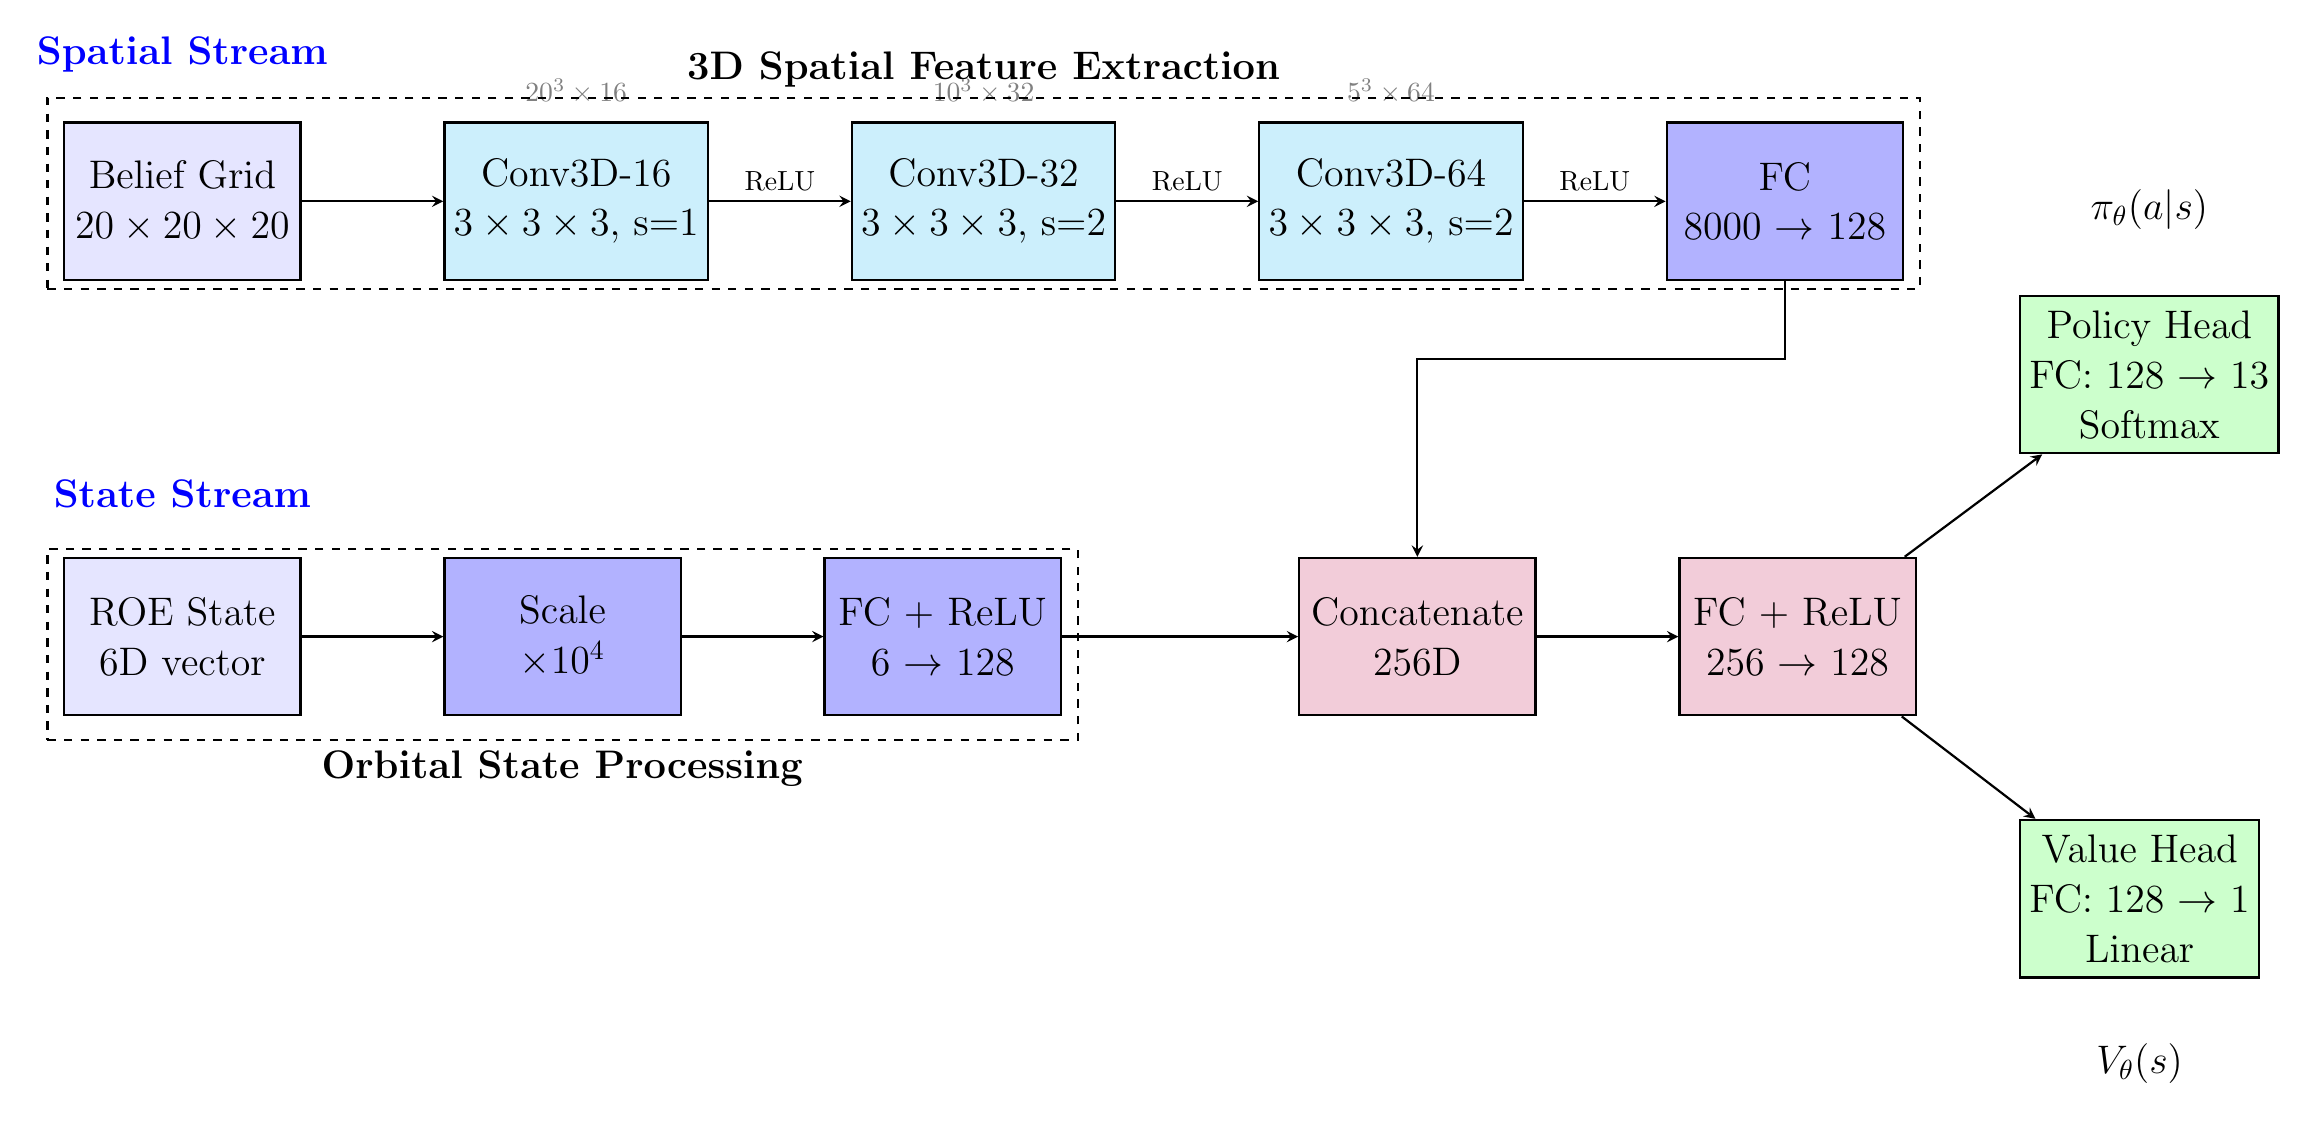
\begin{tikzpicture}[
    node distance=1.5cm,
    box/.style={rectangle, draw, thick, minimum width=3cm, minimum height=2cm, align=center, font=\Large},
    input/.style={box, fill=blue!10},
    conv/.style={box, fill=cyan!20},
    fc/.style={box, fill=blue!30},
    shared/.style={box, fill=purple!20},
    output/.style={box, fill=green!20, minimum width=3cm},
    arrow/.style={->, >=stealth, thick}
]

% Belief Grid Stream (Top)
\node[input] (grid_input) {Belief Grid\\$20 \times 20 \times 20$};
\node[conv, right=of grid_input, xshift=0.3cm] (conv1) {Conv3D-16\\$3 \times 3 \times 3$, s=1};
\node[conv, right=of conv1, xshift=0.3cm] (conv2) {Conv3D-32\\$3 \times 3 \times 3$, s=2};
\node[conv, right=of conv2, xshift=0.3cm] (conv3) {Conv3D-64\\$3 \times 3 \times 3$, s=2};
\node[fc, right=of conv3, xshift=0.3cm] (fc_grid) {FC\\8000 $\rightarrow$ 128};

% ROE Stream (Bottom)
\node[input, below=3cm of grid_input, yshift=-0.5cm] (roe_input) {ROE State\\6D vector};
\node[fc, right=of roe_input, xshift=0.3cm] (scale) {Scale\\$\times 10^4$};
\node[fc, right=of scale, xshift=0.3cm] (fc_roe) {FC + ReLU\\6 $\rightarrow$ 128};

% Shared layers
\node[shared, right=2.5cm of fc_roe, xshift=0.5cm] (concat) {Concatenate\\256D};
\node[shared, right=of concat, xshift=0.3cm] (fc_shared) {FC + ReLU\\256 $\rightarrow$ 128};

% Output heads
\node[output, above right=1cm and 1cm of fc_shared, xshift=0.3cm, yshift=0.3cm] (policy) {Policy Head\\FC: 128 $\rightarrow$ 13\\Softmax};
\node[output, below right=1cm and 1cm of fc_shared, xshift=0.3cm, yshift=-0.3cm] (value) {Value Head\\FC: 128 $\rightarrow$ 1\\Linear};

% Arrows - Grid stream
\draw[arrow] (grid_input) -- (conv1);
\draw[arrow] (conv1) -- node[above, font=\normalsize] {ReLU} (conv2);
\draw[arrow] (conv2) -- node[above, font=\normalsize] {ReLU} (conv3);
\draw[arrow] (conv3) -- node[above, font=\normalsize] {ReLU} (fc_grid);

% Arrows - ROE stream
\draw[arrow] (roe_input) -- (scale);
\draw[arrow] (scale) -- (fc_roe);

% Arrows - Convergence
\draw[arrow] (fc_grid) -- ++(0,-2) -| (concat);
\draw[arrow] (fc_roe) -- (concat);
\draw[arrow] (concat) -- (fc_shared);

% Arrows - Output
\draw[arrow] (fc_shared) -- (policy);
\draw[arrow] (fc_shared) -- (value);

% Dimension annotations
\node[above=0.1cm of conv1, font=\normalsize, text=gray] {$20^3 \times 16$};
\node[above=0.1cm of conv2, font=\normalsize, text=gray] {$10^3 \times 32$};
\node[above=0.1cm of conv3, font=\normalsize, text=gray] {$5^3 \times 64$};

% Stream labels
\node[above=0.3cm of grid_input, font=\Large\bfseries, text=blue, yshift=0.2cm] {Spatial Stream};
\node[above=0.3cm of roe_input, font=\Large\bfseries, text=blue, yshift=0.2cm] {State Stream};

% Final outputs
\node[above=0.5cm of policy, font=\Large, yshift=0.2cm] {$\pi_\theta(a|s)$};
\node[below=0.5cm of value, font=\Large, yshift=-0.2cm] {$V_\theta(s)$};

% Add bounding boxes for clarity
\node[draw, dashed, thick, fit=(grid_input) (conv1) (conv2) (conv3) (fc_grid),
      label=above:{\Large\textbf{3D Spatial Feature Extraction}}, inner sep=0.2cm, yshift=0.1cm] {};
\node[draw, dashed, thick, fit=(roe_input) (scale) (fc_roe),
      label=below:{\Large\textbf{Orbital State Processing}}, inner sep=0.2cm, yshift=-0.1cm] {};

\end{tikzpicture}

\end{document}
